




\section{Exploración Univariada}\label{univariada}

En esta sección nos interesa explorar cada indice (IDH), para esto se realizan varias estadisticas con la información obtenida. En primer lugar, se evalua el numero de datos y la mediana de cada uno de los tipos de población.




% Table created by stargazer v.5.2.2 by Marek Hlavac, Harvard University. E-mail: hlavac at fas.harvard.edu
<<<<<<< HEAD
% Date and time: Fri, Jun 29, 2018 - 7:51:26 PM
=======
% Date and time: vie, jun 29, 2018 - 07:26:33 p.m.
>>>>>>> 0dfb99868056277324f1b1ce6d1f735f46219494
\begin{table}[!htbp] \centering 
  \caption{Medidas estadísticas} 
  \label{stats} 
\begin{tabular}{@{\extracolsep{5pt}}lcc} 
\\[-1.8ex]\hline 
\hline \\[-1.8ex] 
Statistic & \multicolumn{1}{c}{N} & \multicolumn{1}{c}{Median} \\ 
\hline \\[-1.8ex] 
cabecera & 32 & 717,197 \\ 
resto & 32 & 268,111.5 \\ 
\hline \\[-1.8ex] 
\end{tabular} 
\end{table} 
Para resaltar lo anterior, tenemos la Figura \ref{histograma} en la página \pageref{histograma}. 


%%%%% figure
\begin{figure}[h]
\centering
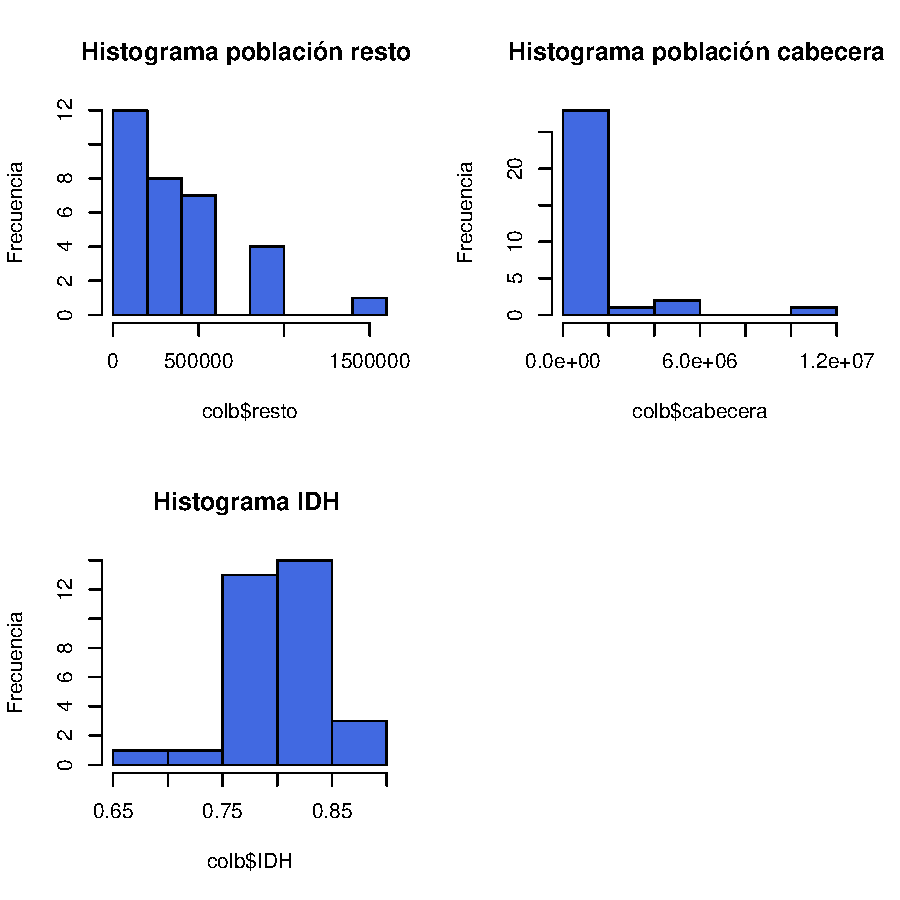
\includegraphics{Paper-histograma}
\caption{Histograma del IDH }
\label{histograma}
\end{figure}


Como las poblaciones tienen un sesgo se normalizan los datos con log, el histograma de estos nuevos datos se muestra en la Figura \ref{normalizados} en la página \pageref{normalizados}.

\begin{figure}[h]
\centering
\begin{adjustbox}{height=4cm}
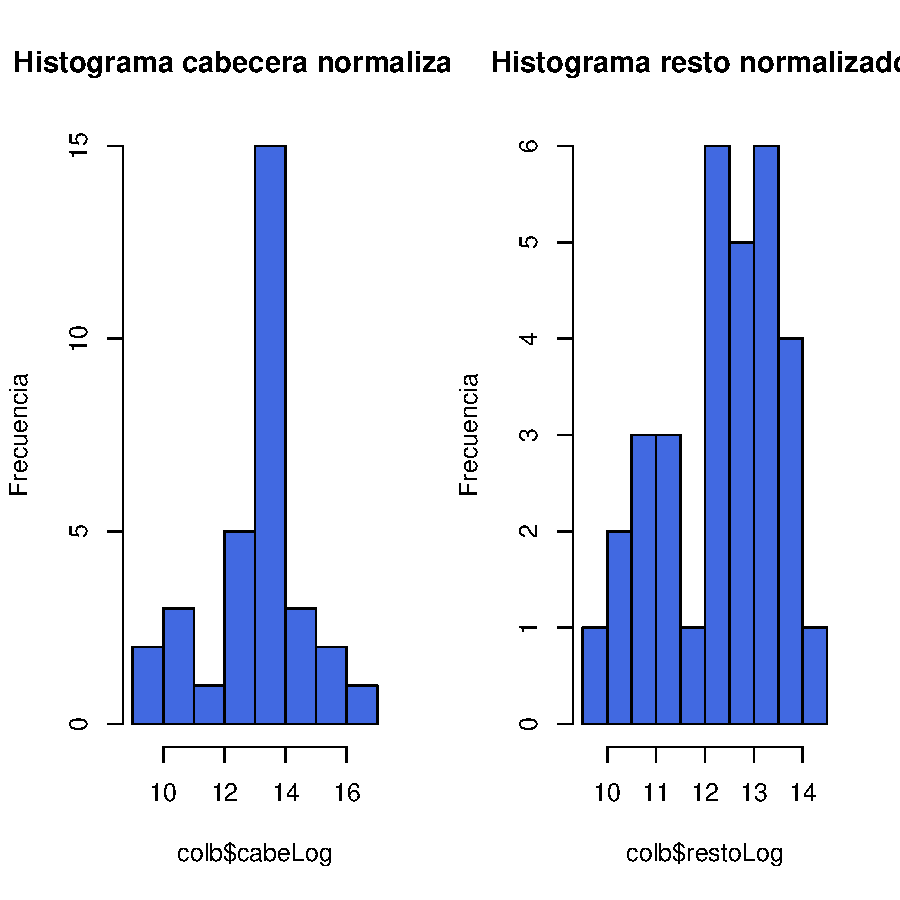
\includegraphics{Paper-004}
\end{adjustbox}
\caption{Histograma de poblaciones }
\label{normalizados}
\end{figure}


\section{Exploración Bivariada}\label{bivariada}

en esta sección nos interesa ver el impacto que tiene la población en el IDH, para esto se presenta en la tabla \ref{corrDem} en la página \pageref{corrDem}. la correlación de las variables normalizadas con respecto al IDH


% Table created by stargazer v.5.2.2 by Marek Hlavac, Harvard University. E-mail: hlavac at fas.harvard.edu
<<<<<<< HEAD
% Date and time: Fri, Jun 29, 2018 - 7:51:33 PM
=======
% Date and time: vie, jun 29, 2018 - 07:26:38 p.m.
>>>>>>> 0dfb99868056277324f1b1ce6d1f735f46219494
\begin{table}[!htbp] \centering 
  \caption{Correlación de Democracia con las demás variables} 
  \label{corrDem} 
\begin{tabular}{@{\extracolsep{5pt}} cc} 
\\[-1.8ex]\hline 
\hline \\[-1.8ex] 
total & cabeLog \\ 
\hline \\[-1.8ex] 
$0.399$ & $0.487$ \\ 
\hline \\[-1.8ex] 
\end{tabular} 
\end{table} 


Ademas, se muestra la correlacion entre todas las variables independientes en la tabla \ref{corrTableX} en la página \pageref{corrTableX}

% Table created by stargazer v.5.2.2 by Marek Hlavac, Harvard University. E-mail: hlavac at fas.harvard.edu
<<<<<<< HEAD
% Date and time: Fri, Jun 29, 2018 - 7:51:33 PM
=======
% Date and time: vie, jun 29, 2018 - 07:26:38 p.m.
>>>>>>> 0dfb99868056277324f1b1ce6d1f735f46219494
\begin{table}[!htbp] \centering 
  \caption{Correlación entre variables independientes} 
  \label{corrTableX} 
\begin{tabular}{@{\extracolsep{5pt}} ccc} 
\\[-1.8ex]\hline 
\hline \\[-1.8ex] 
 & total & cabeLog \\ 
\hline \\[-1.8ex] 
total & 1 &  \\ 
cabeLog & 0.71 & 1 \\ 
\hline \\[-1.8ex] 
\end{tabular} 
\end{table} 
los datos anteriores los puede ver visualmente en la figura \ref{puntos} en la página \pageref{puntos}

\begin{figure}[h]
\centering
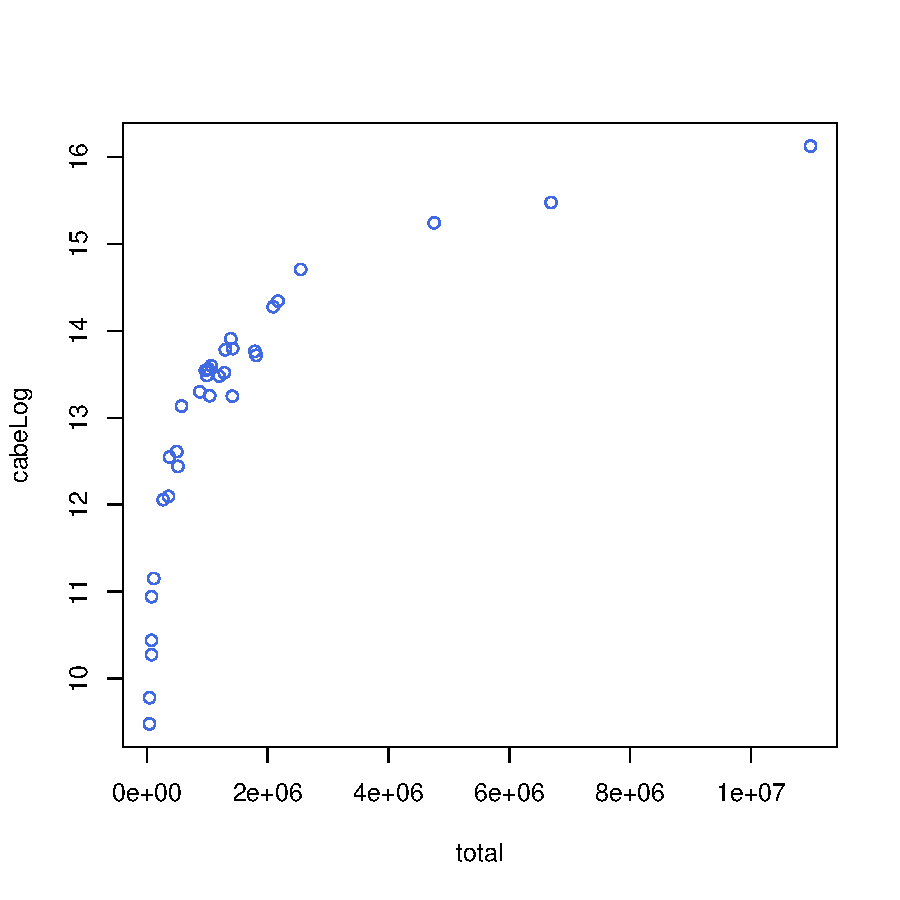
\includegraphics{Paper-puntos}
\caption{correlacion entre cabelog y restolog }
\label{puntos}
\end{figure}




\section{Modelos de Regresión}\label{regresion}

Finalmente, vemos los modelos propuestos. En cada una se evalua la variable independiente DIH con cada una de las categorias de la poblacion. Los resultados se muestran en la Tabla \ref{regresiones} de la página \pageref{regresiones}.


% Table created by stargazer v.5.2.2 by Marek Hlavac, Harvard University. E-mail: hlavac at fas.harvard.edu
<<<<<<< HEAD
% Date and time: Fri, Jun 29, 2018 - 7:51:33 PM
=======
% Date and time: vie, jun 29, 2018 - 07:26:38 p.m.
>>>>>>> 0dfb99868056277324f1b1ce6d1f735f46219494
\begin{table}[!htbp] \centering 
  \caption{Modelos de Regresión} 
  \label{regresiones} 
\begin{tabular}{@{\extracolsep{5pt}}lccc} 
\\[-1.8ex]\hline 
\hline \\[-1.8ex] 
 & \multicolumn{3}{c}{\textit{Dependent variable:}} \\ 
\cline{2-4} 
\\[-1.8ex] & \multicolumn{3}{c}{IDH} \\ 
\\[-1.8ex] & (1) & (2) & (3)\\ 
\hline \\[-1.8ex] 
 cabeLog & 0.013$^{***}$ &  &  \\ 
  & (0.004) &  &  \\ 
  & & & \\ 
 restoLog &  & 0.007 &  \\ 
  &  & (0.007) &  \\ 
  & & & \\ 
 totalLog &  &  & 0.013$^{**}$ \\ 
  &  &  & (0.005) \\ 
  & & & \\ 
 Constant & 0.634$^{***}$ & 0.722$^{***}$ & 0.629$^{***}$ \\ 
  & (0.055) & (0.082) & (0.068) \\ 
  & & & \\ 
\hline \\[-1.8ex] 
Observations & 32 & 32 & 32 \\ 
R$^{2}$ & 0.238 & 0.031 & 0.179 \\ 
Adjusted R$^{2}$ & 0.212 & $-$0.001 & 0.152 \\ 
Residual Std. Error (df = 30) & 0.037 & 0.042 & 0.039 \\ 
F Statistic (df = 1; 30) & 9.347$^{***}$ & 0.974 & 6.561$^{**}$ \\ 
\hline 
\hline \\[-1.8ex] 
\textit{Note:}  & \multicolumn{3}{r}{$^{*}$p$<$0.1; $^{**}$p$<$0.05; $^{***}$p$<$0.01} \\ 
\end{tabular} 
\end{table} 


















\endinput
